\chapter{Návrh}

Tato kapitola popisuje návrh implementace a komplementárních struktur.

\section{Toolbar}

Toolbar je strukturní komponenta, která obsahuje skupinu focusovatelných elementů.

\begin{figure}[htp]
    \centering
    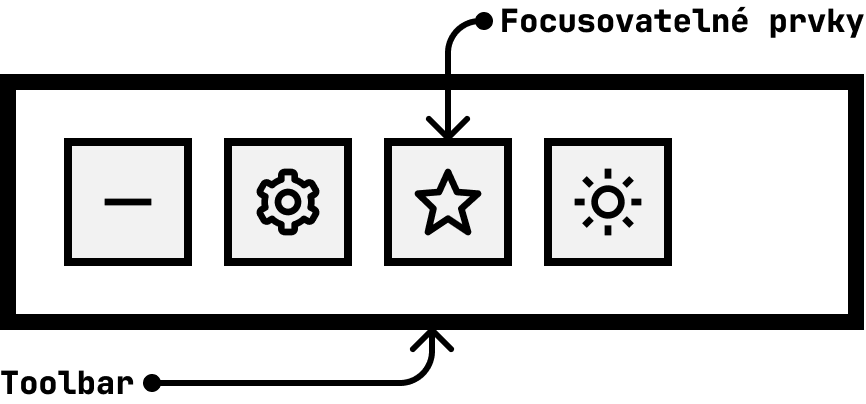
\includegraphics[max size={\linewidth}{\textheight}]{./assets/figures/anatomy/toolbar.png}
    \captionsetup{justification=centering}
    \caption{Low-fidelity wireframe komponenty Toolbar}
\end{figure}

Hlavní přínos této komponenty je jednodušší klávesová navigace pomocí klávesových šipek a dalších zkratek namísto klasického proklikávání tabulátorem.

Pro splnění požadavku \hyperref[ofr11]{\fr{OFR 1.1}} je potřeba splnit následující podmínky:

\begin{enumerate}
    \item Tabulátor směrem dopředu skočí na první, nebo naposled vybraný focusovatelný prvek v rámci Toolbaru.
    \item Tabulátor směrem dopředu, když je focus v rámci Toolbaru, skočí na první focusovatelný prvek mimo Toolbar.
    \item Šipky vlevo a vpravo přesunou focus mezi focusovatelnými prvky v rámci Toolbaru pokud je orientace toolbaru horizontální.
    \item Šipky nahoru a dolů přesunou focus mezi focusovatelnými prvky v rámci Toolbaru pokud je orientace toolbaru vertikální.
    \item Klávesy \texttt{Home} a \texttt{End} přesunou focus na první, respektive poslední focusovatelný prvek v rámci Toolbaru.
\end{enumerate}

\section{SpinButton}

SpinButton je formulářová komponenta, která vymezuje rozsah diskrétních hodnot a typicky umožňuje uživateli změnit její hodnotu pomocí tlačítek snížit a navýšit, nebo alternativně skrze textový vstup.

\begin{figure}[htp]
    \centering
    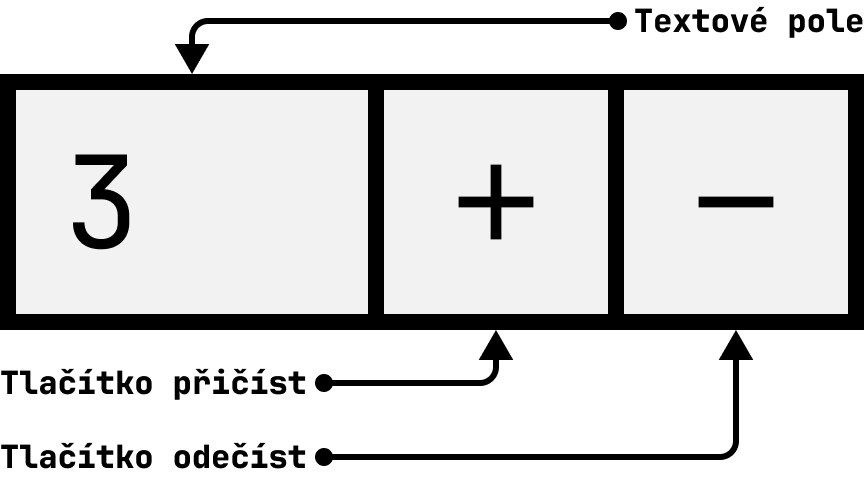
\includegraphics[max size={\linewidth}{\textheight}]{./assets/figures/anatomy/spinbutton.png}
    \captionsetup{justification=centering}
    \caption{Low-fidelity wireframe komponenty SpinButton}
\end{figure}

\section{Carousel}

Carousel je komponenta pro zobrazení multimediálního obsahu v podobě obrázků, videí nebo alternativních prvků.
V rámci \gls{apg} jsou popsané tři varianty této komponenty popsané níže.

\begin{figure}[htp]
    \centering
    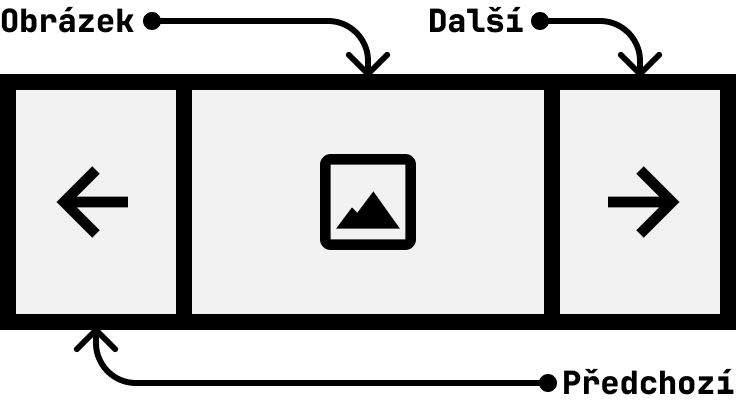
\includegraphics[max size={\linewidth}{\textheight}]{./assets/figures/anatomy/carousel.png}
    \captionsetup{justification=centering}
    \caption{Low-fidelity wireframe komponenty Carousel}
\end{figure}

% \subsection{Basic Carousel}

% TODO

% \subsection{Tabbed Carousel}

% TODO

% \subsection{Grouped Carousel}

% TODO

\section{Dokumentace}

Součástí zadání práce a požadavku \hyperref[nfr14]{\fr{NFR 1.4}} je vytvoření dokumentace pro implementované komponenty.
Dokumentace by měla obsahovat několik zásadních sekcí:

\begin{enumerate}
    \item \textbf{Anatomie komponenty}

          Anatomie by měla popisovat způsob naimportování knihovny, její typovou signaturu a low-fidelity návrh.

    \item \textbf{API referenci}

          \gls{api} reference by měla popisovat vstupní parametry, jejich výchozí hodnoty a typ tak, aby ušetřila čas vývojáři pro pochopení implementace.

    \item \textbf{Příklad}

          Příklad by měl být vnořený na stránce tak, aby komponentu šlo používat jako v normální aplikaci. Součástí příkladu by měl jeho kopírovatelný zdrojový kód.

    \item \textbf{Ukázka s odečítačem obrazovky}

          V dokumentaci by měla být i ukázka toho, jak komponenta reaguje na použití s odečítačem obrazovky.

\end{enumerate}

Kromě výše zmíněných částí u každé stránky s komponentou by měla dokumentace obsahovat informace o tom, jak knihovnu nainstalovat a které technologie je potřeba mít nainstalovené.
V neposlední řadě by měla dokumentace obsahovat odkazy na informaci o implementovaném návrhovém vzoru, výsledky testů a pokrytí kódu testy.
